\documentclass[12pt]{article}
\usepackage[a4paper, left=25mm, right=25mm]{geometry}
\usepackage{polski}
\usepackage{graphicx}
\usepackage{caption}
\graphicspath{ {./images/} }
\usepackage{hyperref}
% \usepackage[T1]{fontenc}
\usepackage{mathptmx}
\usepackage{tocloft}
\usepackage{booktabs} % Pakiet do lepszego formatowania tabeli
\usepackage{tabularx}
\usepackage{amssymb}
% \usepackage{tocloft}
% \usepackage[ natbib=true, style=numeric,sorting=none]{biblatex}
% \usepackage[natbib=true, style=numeric,sorting=none, maxnames=2, uniquelist=false]{biblatex}
% \addbibresource{biblio.bib}



% \renewcommand\cftsecfont{\normalfont}
\renewcommand\cftsecpagefont{\normalfont}
\renewcommand{\cftsecleader}{\cftdotfill{\cftsecdotsep}}
\renewcommand\cftsecdotsep{\cftdot}
\renewcommand\cftsubsecdotsep{\cftdot}
\renewcommand\cftsubsubsecdotsep{\cftdot}

\begin{document}
\begin{titlepage}
    \begin{center}
    
    
\includegraphics[width=0.8\textwidth]{logo}
    \vspace*{1cm}

        \Huge
        \textbf{Inżynieria Systemów Informatycznych}
 
        \vspace{0.5cm}
        \Large
        System biblioteki
             
        \vspace{1.5cm}
 
        \textbf{Autorzy:}   \\ Adam Drożdż w69555 \\
                            Bartłomiej Kieroński w62951 \\
                            Dawid Niezgoda w58968 \\
                            Mateusz Frużyński w69560

        \vspace*{1cm}
        \textbf{Prowadzący:} \\ Dr inż. Maksymilian Knap
 
        \vfill
            
        \today
             
    \end{center}
 \end{titlepage}

\tableofcontents
\addtocounter{page}{1}

\newpage
\section{Opis systemu}
Nie każda osoba lubiąca czytać książki musi je kupować w księgarni. Istnieje wiele przyczyn, przez które lepszym rozwiązaniem jest wypożyczanie książek w~bibliotece. Jednymi z takich przyczyn może być ogólna brak dostępności wybranych pozycji w~księgarni lub nie wystarczającej ilości miejsca na biblioteczkę w mieszkaniu. Biblioteki spełnią ważne funkcje dla społeczeństwa. Daje ona szansę na pozyskiwanie wiedzy z~różnych dziedzin. Przez zwiekszenie czytelnictwa, zwiększa się zasób słownictwa jak i~wiedzy czytelników. Zwiekszenie zasobu słownictwa jak i~wiedzy pozwala na elokwentne wypowiedzi na wiele tematów. 

W bibliotece zorganizowanej bez systemu informatycznego wszystkie dane muszą być przechowywane w szafkach oraz segregatorach. Używanie takiej bazy danych jet stosunkowo mało efektywne. Bibliotekarze którzy chcą sprawdzić dostępność książki, musą ręcznie przeszukać segregatory. Innym problemem w takim systemie jest trudność w~przechowywaniu takiej bazy danych. Szafki z segregatorami zajmują dużo miejsca, przez co często nie ma gdzie jch przechowywać. Podobny problem odnosi się do tworzenia kopi zapasowej. Tworzenie kopi zapasowej takiej bazy danych jest bardzo czasochłonne. Po stworzeniu tej kopi, nasuwa się pytanie co zrobić z już nieaktualną kopią danych? Przechowywanie takich kopi zajmuje dużo miejsca, dla tego taka biblioteka nie będzie w stanie przechowywane takich kopi. Natomiast usunięcie starch kopi zapasowych jest kosztowne i~czasochłonne. Najwygodniejszym rozwiązaniem było by nie wykonywanie kopi zapasowych danych, ale czy jest to rozsądne?

Przejscie na system informatyczny przynosi wiele korzyści. Nie jest wymagane miejsce na przechlanie danych w~forme segregatorów. Poprzez zwolnienie miejsca które było wykorzystane do przechowywania danych, można zwiększyć ilość dostępnych książek w~księgarni. Następną korzyścią jest możliwość wygodnego przechowywania jak i zażądanie kopią zapasową bazy danych. Po za tym, za pomoca systemu informatycznego jest możliwość powiadomienie użytkownika o~zbliżającym terminie oddania książki, przedłużenie wypozyczenia książki, zarezerwowanie konkretnej książki itp. System informatyczny pozwala te wszystkie czynności wykonywać za pomoca aplikacji internetowa. Do korzystania z~tej aplikacji wystarczy dostęp do internetu oraz przeglądarka internetowa. Jest to wygody sposób do korzystania z~tego systemu prze użytkownika.

\section{Fukcjonalności systemu}
\begin{enumerate}
    \item System przechowuje informacje o dostępnych książkach, ich autorach, numerach ISBN, wydawcach, kategoriach i dostępności.
    \item System dodaje nowe pozycje do katalogu.
    \item System umożliwia użytkownikom wypożyczanie książek z biblioteki poprzez zapisywanie informacji o wypożyczonych pozycjach.
    \item System pozwala czytelnikom rezerwować książki, które są aktualnie niedostępne, umożliwiając im otrzymanie powiadomienia, gdy pozycja zostanie zwrócona i będzie ponownie dostępna.
    \item System może obsługiwać zasoby cyfrowe, takie jak e-booki, artykuły elektroniczne czy audiobooki, umożliwiając ich wypożyczanie lub dostęp online.
    \item System umożliwia czytelnikom dodawanie recenzji oraz ocenianie książek, co pomaga innym w wyborze odpowiednich pozycji.
    \item System umożliwia genetowanie raportów dotyczących popularności książek, aktywności czytelników, trendów czy wolumenu wypożyczeń. To przydatne narzędzie do planowania zakupów nowych książek.
    \item System umożliwia obsługę wielu oddziałó, system może integrować zarządzanie wszystkimi lokalizacjami, umożliwiając np. transfer książęk między nimi.
    \item System umożliwia obsługę opłat za kary, usługi czy też zakupy książek przez czytelników.
    \item Interfejs dla pracowników i czytelników zapewnia łatwy dostęp do systemu zarówno dla pracowników obsługujących bibliotekę, jak i dla czytelników korzystających z usług.
\end{enumerate}
\newpage
\section{Diagram DFD}
\begin{figure}[!h]
    \centering
    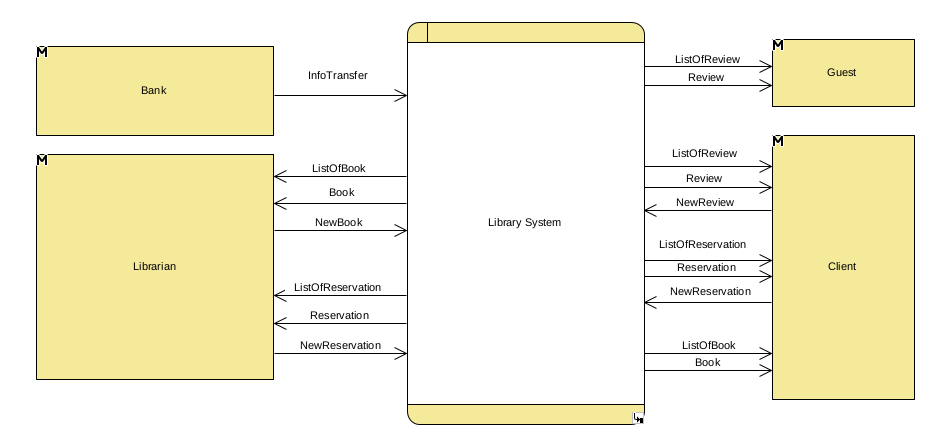
\includegraphics[width=0.75\textwidth]{Schemat}
    \caption{Diagram DFD  poziomu 0 dla biblioteki.}
\end{figure}


\begin{figure}[!h]
    \centering
    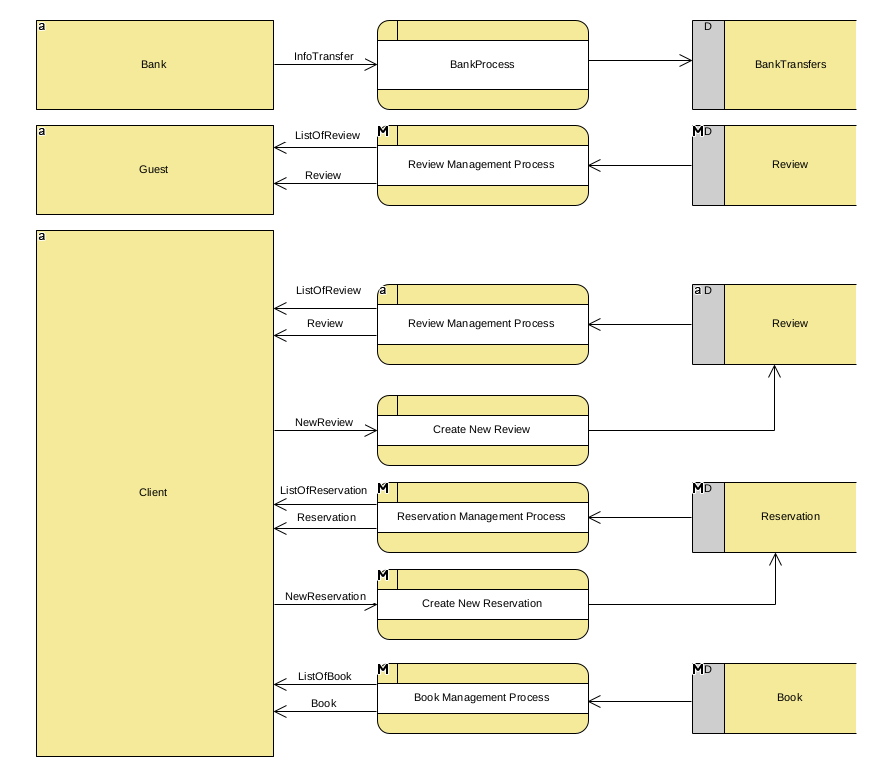
\includegraphics[width=0.75\textwidth]{Schemat2}
    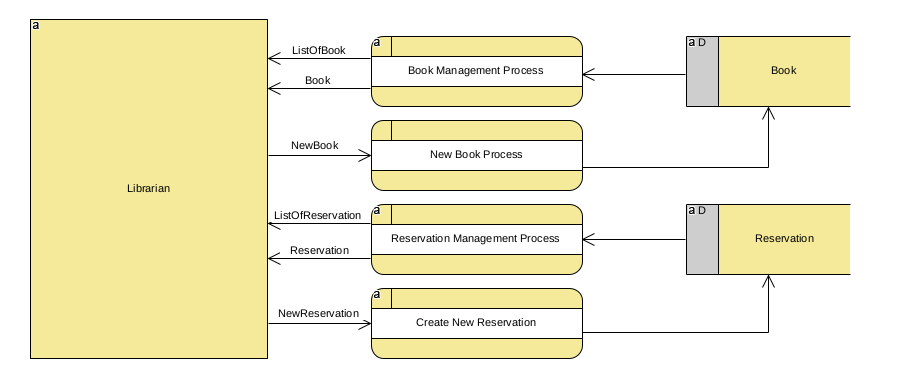
\includegraphics[width=0.75\textwidth]{Schemat3}
    \caption{Diagram DFD poziomu 1 dla dla biblioteki.}
\end{figure}

\end{document}